\documentclass{article}
\usepackage{amsmath,amssymb,graphicx,algpseudocode,algorithm,amsthm}
\usepackage[margin=1in]{geometry}
\usepackage{mathrsfs}
\let\mathcrl\mathscr
\usepackage[mathscr]{euscript}
\usepackage{marginnote}
\usepackage{hyperref}
\usepackage{qtree}
\usepackage{graphicx}
\usepackage{tikz}
\geometry{reversemarginpar}


\author{Benji Altman}

\def\latex{\LaTeX\ }

\def\useLim{\limits}
\newcommand{\question}[1]{\marginnote{#1}}
\let\union\cup
\let\inter\cap
\let\emptyset\varnothing
\let\bigunion\bigcup
\let\biginter\bigcap
\let\composed\circ
\let\cross\times
\def\And{\textit{ and }}
\def\Or{\textit{ or }}
\def\sbSeperator{\,\middle|\,}
\def\Return{\State\textbf{return}\par}
\def\ZNonNegative{{\mathbb Z_{\ge 0}}}
\newcommand{\setcomp}[1]{{#1}^{\mathsf{c}}}
\newcommand{\prodfrom}[3]{\prod\useLim_{#1}^{#2}\LB {#3} \RB}
\newcommand{\sumfrom}[3]{\sum\useLim_{#1}^{#2} \LB {#3} \RB}
\newcommand{\unionfrom}[3]{\bigunion\useLim_{#1}^{#2} \LB {#3} \RB}
\newcommand{\interfrom}[3]{\biginter\useLim_{#1}^{#2} \LB {#3} \RB}
\newcommand{\interacross}[2]{\interfrom{#1}{}{#2}}
\newcommand{\unionacross}[2]{\unionfrom{#1}{}{#2}}
\newcommand{\sumacross}[2]{\sumfrom{#1}{}{#2}}
\newcommand{\prodacross}[2]{\prodfrom{#1}{}{#2}}
\newcommand{\Lim}[3]{\lim\useLim_{{#1} \to {#2}}\LB {#3} \RB}
\newcommand{\set}[1]{\left\{ {#1} \right\}}
\newcommand{\setbuilder}[2]{\left\{{#1} \sbSeperator {#2}\right\}}
\newcommand{\derivative}[2]{\frac{d}{d{#2}}\LB {#1} \RB}
\newcommand{\Exists}[2]{\exists_{#1}\LB {#2} \RB}
\newcommand{\All}[2]{\forall_{#1}\LB {#2} \RB}
\newcommand{\abs}[1]{\left|{#1}\right|}
\newcommand{\card}[1]{\left| {#1} \right|}
\newcommand{\range}[1]{\textit{\textbf{Rng}}\left( {#1} \right)}
\newcommand{\domain}[1]{\textit{\textbf{Dom}}\left( {#1} \right)}
\newcommand{\pset}[1]{\mathcal P\left( {#1} \right)}
\newcommand{\pair}[2]{\left( {#1} , {#2} \right)}
\def\closure{\overline}
\newcommand{\limpts}[1]{{#1} '}
\newcommand{\ooint}[2]{\left( {#1} , {#2} \right)}
\newcommand{\ocint}[2]{\left( {#1} , {#2} \right]}
\newcommand{\coint}[2]{\left[ {#1} , {#2} \right)}
\newcommand{\ccint}[2]{\left[ {#1} , {#2} \right]}
\newcommand{\eqclass}[1]{\bar{#1}}
\newcommand{\ceil}[1]{\left\lceil {#1} \right\rceil}
\newcommand{\floor}[1]{\left\lfloor {#1} \right\rfloor}
\newcommand{\inv}[1]{{#1}^{-1}}
\def\true{\text{True}}
\def\false{\text{False}}
\newcommand{\ball}[2]{B_{#1}\left({#2}\right)}
\def\LB{}
\def\RB{}
\newcommand{\cannonicalSet}[1]{\left[ #1 \right]}
\let\lxor\oplus
\newcommand{\norm}[1]{\left|\left|{#1}\right|\right|}

\newtheorem{theorem}{Theorem}[section]
\newtheorem{lemma}[theorem]{Lemma}
\theoremstyle{definition}
\newtheorem{definition}{Definition}[section]

\def\sbSeperator{\ |\ }
\usepackage[toc,xindy]{glossaries}

\makenoidxglossaries

\newglossaryentry{set}
{
	name={set},
	description={A collection of objects}
}
\newglossaryentry{vertex}
{
	name={vertex},
	description={A point or node in a graph},
	plural={verticies}
}
\newglossaryentry{edge}
{
	name={edge},
	description={A connection or line between verticies in a graph}
}
\newglossaryentry{connected}
{
	name={connected},
	description={A graph where one may start at any point and could follow edges and eventually get to any other point}
}
\newglossaryentry{multigraph}
{
	name={multigraph},
	description={Like a graph, but multiple edges may connect the same vertex pair, and an edge may connect a vertex to itself}
}
\newglossaryentry{complete}
{
	name={complete graph},
	description={A graph with all possible edges included, the notation $K_n$ is used to denote the complete with $n$ verticies}
}
\newglossaryentry{face}
{
	name={face},
	description={An section of the space we are embedding our graph in that is separated from the rest of the space by edges}
}
\newglossaryentry{contraction}
{
	name={contraction},
	description={A graph operation where one removes an edge by fusing two verticies together}
}
\newglossaryentry{subgraph}
{
	name={subgraph},
	description={$A$ is a subgraph of some graph $\mathcal G$ iff you could add verticies and edges to $A$ and somehow get $\mathcal G$}
}
\newglossaryentry{graph}
{
	name={graph},
	description={A set of verticies and edges}
}
\title{Topological Graph Theory}
\begin{document}
\maketitle
\tableofcontents



\section{Introduction}
Topological graph theory is an entire field within topology and as such this paper is by no means meant to cover all of topological graph theory in any depth. This paper instead will first cover a rather shallow overview of the field, followed by a more in depth study of graphs and their genus. The overview will mainly be focused on giving a thorough understanding of what topological graph theory is as well as to briefly cover the history of the field. In giving an overview of the field we will cover some of the basic concepts and definitions needed for the more rigorous part of the paper. After the overview we will dive into Kuratowski's Theorem, We will go through and attempt to have an intuitive understanding of a Kuratowski's Theorem and it's proof. After proving Kuratowski's Theorem, we will continue onto talking about generalizations of the theorem and map colorings, however their coverage will be rather shallow and lacking proofs.

\section{Overview}
\subsection{Graphs}
Before we talk about topological graph theory with any level of understanding we must first understand what a \gls{graph} is.

A \gls{graph} is generally defined as a \gls{set} of \glspl{vertex} combined with a \gls{set} of \glspl{edge} between \glspl{vertex}, however here it may be more useful to think about them visually with a simple representation.

Consider first a \gls{set} of points, this may be thought of as just drawing dots on a sheet of paper. Each of these points will be called a \gls{vertex}. Now we may start drawing lines between \glspl{vertex}. Lines may cross over each other and need not be straight. There is no requirement that all \glspl{vertex} have a line going to it. Each of these lines are called an \gls{edge}. We will simply insist that no \gls{edge} connects two \glspl{vertex} and that we do not have multiple \glspl{edge} between the same pair of \glspl{vertex}.

Once we have drawn this we have a representation of a \gls{graph}. If we were to move the \glspl{vertex} around on the paper but leave them having the same \glspl{edge} (the same \glspl{vertex} are connected to the point as they were before). we would be left with the same \gls{graph}. That is to say, it doesn't mater where we put a \gls{vertex} on our sheet, the \gls{graph} exists independently of the representation we draw.

\subsection{K\"onigsberg, and it's seven bridges}

Consider the following photo-realistic drawing of the city of K\"onigsberg.

\input{Konigsberg.pdf_tex}

Now the question is, if we get to choose where we start, can we go for a stroll and cross every bridge exactly once?

I first came across this question in the 8\textsuperscript{th} grade, and it was presented to us during geometry class. While undoubtedly an interesting problem, it is quite misleading to try and think of this as a geometry problem. Instead we will try and reduce it to a \gls{graph} problem.

Let us start by thinking of every island as a \gls{vertex} and every bridge as an \gls{edge}. We find the following \gls{graph}.

\begin{center}
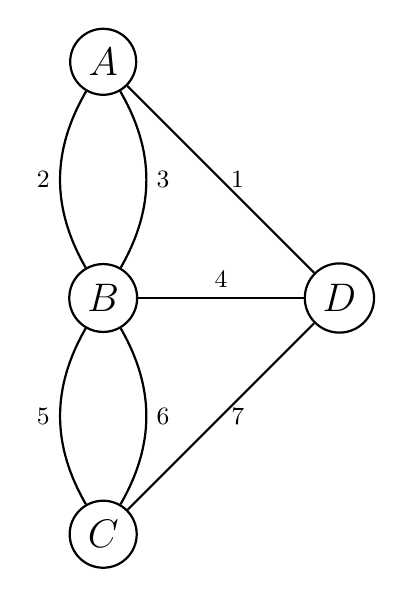
\begin{tikzpicture}[auto, node distance=3cm, every loop/.style={},
                    thick,main node/.style={circle,draw,font=\sffamily\Large\bfseries}]

  \node[main node] (1) {$A$};
  \node[main node] (2) [below of=1] {$B$};
  \node[main node] (3) [below of=2] {$C$};
  \node[main node] (4) [right of=2] {$D$};

  \path[every node/.style={font=\sffamily\small}]
    (1) edge node [right] {$1$} (4)
        edge [bend right] node[left] {$2$} (2)
    (2) edge [bend right] node [right] {$3$} (1)
        edge node {$4$} (4)
        edge [bend right] node[left] {$5$} (3)
    (3) edge [bend right] node [right] {$6$} (2)
    (4) edge node [right] {$7$} (3);
\end{tikzpicture}
\end{center}

It is worth noting two things about the above diagram. First that the labels on the \glspl{vertex} and \glspl{edge} are unrelated to the problem, but have been added simply to make referring to parts of the \gls{graph} much easier. Second that whatever the above image depicts, does not fit our definition of a \gls{graph}.

Notice that \gls{edge} $2$ and \gls{edge} $3$ both connect \gls{vertex} $A$ to $B$, as well \glspl{edge} $5$ and $6$ do for $B$ and $C$. This is a strict violation of our definition for a \gls{graph}. The issue of course then comes to what would one call such a beast as this where, presumably, one is able to have as many connections between any pair of \glspl{vertex} and could even have connections from a \gls{vertex} to itself.

I am particularly glad that you're paying enough attention to notice that the diagram does not depict a \gls{graph}. This is what we will refer to as a \gls{multigraph}. It is worth noting that \glspl{graph} are a type of \gls{multigraph}, so anything we show to be true for all \glspl{multigraph}, is also true for all \glspl{graph}.

Now to solve this problem we need to make one simple observation about how we walk. If we are to go to island (or vertex) we must also leave that island, unless it is the last island we arrive on. This means, that with the exception of the island we start on and end on, each island must have an even number of bridges connected to it. On the \gls{multigraph} we would say that we need all \glspl{vertex} but a start and end \gls{vertex} to have an even number of edges. If we look at the \gls{multigraph} above, we have four \glspl{vertex} that have an odd number of \glspl{edge} connected to them.

\subsection{History}
%TODO add more to section
The seven bridges of K\"onigsberg problem was solved by Euler %TODO Citation (wikipedia for seven bridges of konigsberg)
in 1736. In mathematics this problem is of great historical significance as it is considered to be the beginning of graph theory as well as a sort of precursor to topology. %TODO Citation 

\section{Graph Theory Background}

\subsection{Planer Graphs}

Consider the following \gls{graph}.

\begin{center}
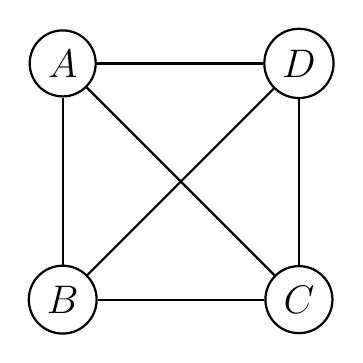
\begin{tikzpicture}[auto, node distance=3cm, every loop/.style={},
                    thick,main node/.style={circle,draw,font=\sffamily\Large\bfseries}]

  \node[main node] (1) {$A$};
  \node[main node] (2) [below of=1] {$B$};
  \node[main node] (3) [right of=2] {$C$};
  \node[main node] (4) [right of=1] {$D$};

  \path[every node/.style={font=\sffamily\small}]
    (1) edge node {} (4)
    	edge node {} (3)
    (2) edge node {} (1)
        edge node {} (4)
    (3) edge node {} (2)
    (4) edge node {} (3);
\end{tikzpicture}
\end{center}

This \gls{graph} is called a \gls{complete} as every \gls{vertex} is connected to every other \gls{vertex} by an \gls{edge}; in fact this \gls{graph} in particular is called $K_4$ as it is the complete four vertex \gls{graph}. We would like to find out if we can draw this above \gls{graph} without having any lines crossing. We can in fact draw this \gls{graph} without any intersections and for any skeptics who may being reading this, the below is $K_4$ without any \glspl{edge} intersecting.

\begin{center}
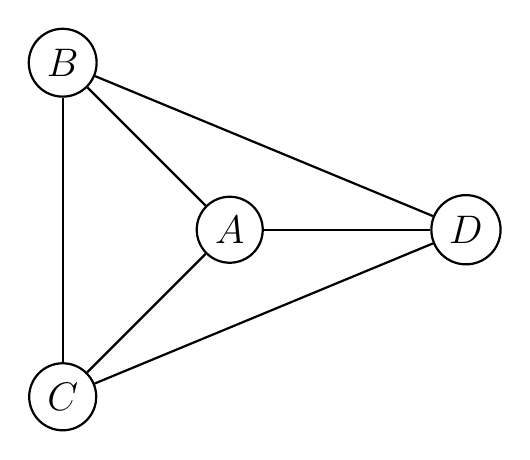
\begin{tikzpicture}[auto, node distance=3cm, every loop/.style={},
                    thick,main node/.style={circle,draw,font=\sffamily\Large\bfseries}]

  \node[main node] (1) {$A$};
  \node[main node] (2) [above left of=1] {$B$};
  \node[main node] (3) [below left of=1] {$C$};
  \node[main node] (4) [right of=1] {$D$};

  \path[every node/.style={font=\sffamily\small}]
    (1) edge node {} (4)
    	edge node {} (3)
    (2) edge node {} (1)
        edge node {} (4)
    (3) edge node {} (2)
    (4) edge node {} (3);
\end{tikzpicture}
\end{center}

So if this \gls{graph} can be drawn without intersection, can any \gls{graph} be drawn without intersections? If some can and some can't how do we tell which can be drawn and which can not? The answer to this comes in Kuratowski's theorem, however before we can even state this theorem we need to build up a bit of terminology for graph theory.

\subsection{Graph Drawing}
A graph drawing is exactly what it sounds like. We've already seen drawings of graphs like the one for K\"oingsberg and two drawings of $k_4$, this means there may be multiple distinct drawings for the same graph. Now we don't need to be very worried about what defines a drawing, that won't be important to us. Simply think of it as the drawing.

If a drawing has no edges intersecting it is said to be a plane drawing. If there exists such a drawing for a particular graph, then that graph is a planar graph.

\subsection{Face}
Faces are a bit of an odd property here as they fundamentally are actually properties only of plane drawings and not graphs themselves; however the number of faces, as we will see stays consistent between any plane drawing of a planar graph and as such the number of faces is a property that planar graphs have.

A face is defined as a connected space that contains no edges or verticies and itself is bounded by edges and verticies.

If you think back to high-school geometry and cubes you may recall that a each of the corners is a vertex, the lines connecting verticies are edges and the area between the edges are faces. In a graph we have verticies connected by edges and when we draw them there are empty areas enclosed by edges and verticies. For example the following would correspond with a cube
\begin{center}
	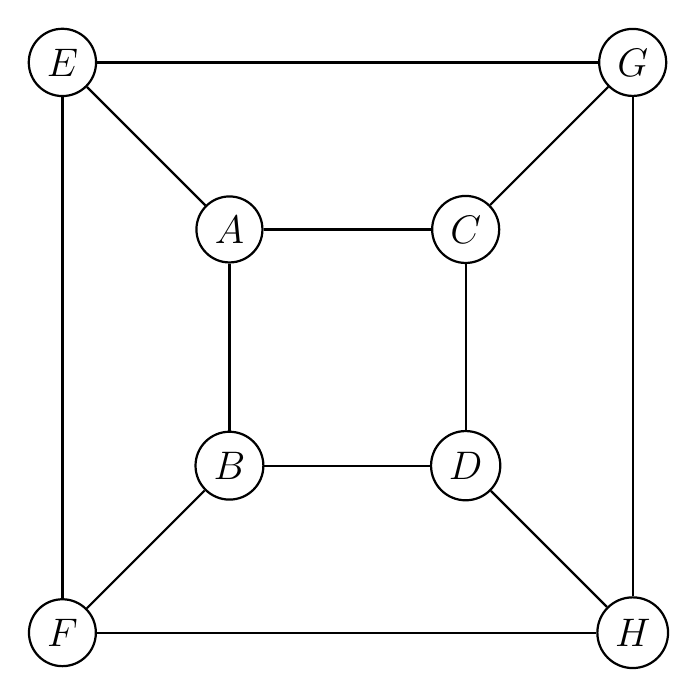
\begin{tikzpicture}[auto, node distance=3cm, every loop/.style={},
	thick,main node/.style={circle,draw,font=\sffamily\Large\bfseries}]
	
	\node[main node] (1) {$A$};
	\node[main node] (2) [below of=1] {$B$};
	\node[main node] (3) [right of=1] {$C$};
	\node[main node] (4) [right of=2] {$D$};
	\node[main node] (5) [above left of=1] {$E$};
	\node[main node] (6) [below left of=2] {$F$};
	\node[main node] (7) [above right of=3] {$G$};
	\node[main node] (8) [below right of=4] {$H$};
	
	\path[every node/.style={font=\sffamily\small}]
	(1) edge node {} (2)
	edge node {} (3)
	edge node {} (5)
	(2) edge node {} (4)
	edge node {} (6)
	(3) edge node {} (4)
	edge node {} (7)
	(4) edge node {} (8)
	(5) edge node {} (6)
	edge node {} (7)
	(6) edge node {} (8)
	(7) edge node {} (8);
	\end{tikzpicture}
\end{center}
Now we can imagine that if we look at the cube straight on maybe $ABDC$ would be the face we are looking at. So too we see the area enclosed in $ABDC$ is a face by the definition we gave. The same is true for $ABFE$, $ACGE$, $DBFH$, and $DCGH$, however that leaves us with only five faces on this cube. The last face must logically come from $EFHG$, however the area enclosed by that contains all the other edges and verticies, so it doesn't fit our definition. However we may notice that the infinite space outside $EFHG$ does not contain any verticies, and therefore we get a sixth face.

Consider then the following very simple graph:
\begin{center}
	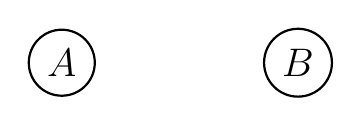
\begin{tikzpicture}[auto, node distance=3cm, every loop/.style={},
	thick,main node/.style={circle,draw,font=\sffamily\Large\bfseries}]
	
	\node[main node] (1) {$A$};
	\node[main node] (2) [right of=1] {$B$};
	
	
	\end{tikzpicture}
\end{center}
Now we still only have one face, however it doesn't have as nice a boundary as they did in the cube. However if we look at all of space excluding $A$ and $B$ then we still get a valid space by our definition.

\subsection{Path}
Now moving onto a more traditional graph property we have the concept of a path. A path is defined as a finite sequence of verticies with the property that each element of the sequence (excluding the last one) has an edge from it to the next element. For example consider the following graph.

\begin{center}
	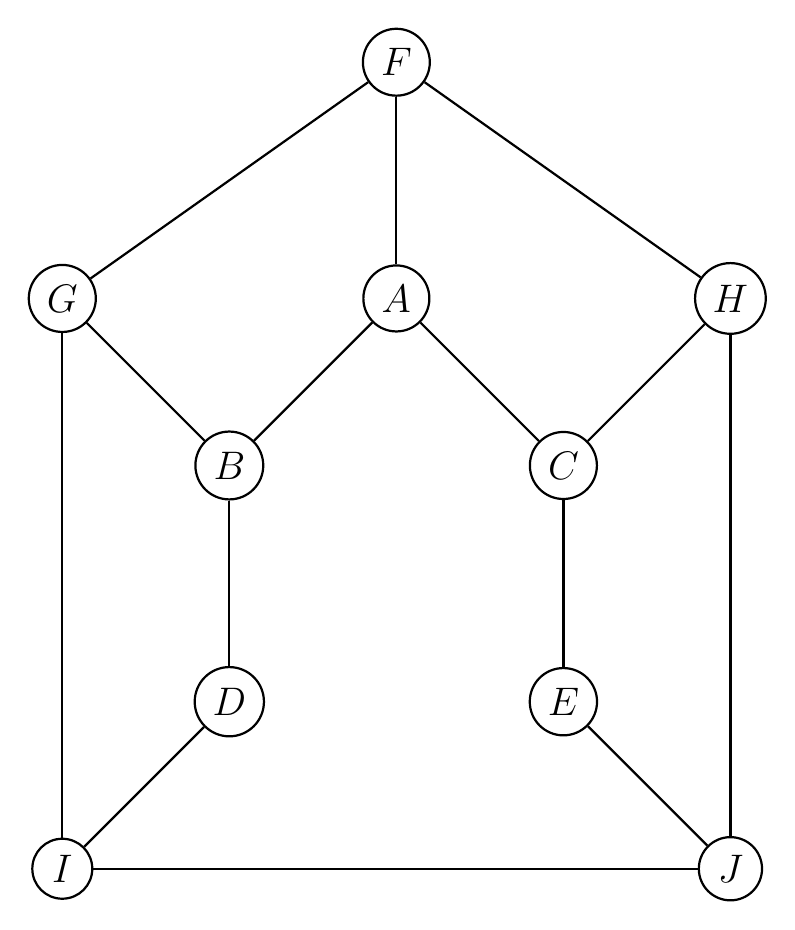
\begin{tikzpicture}[auto, node distance=3cm, every loop/.style={},
	thick,main node/.style={circle,draw,font=\sffamily\Large\bfseries}]
	
	\node[main node] (a) {$A$};
	\node[main node] (b) [below left of=a] {$B$};
	\node[main node] (c) [below right of=a] {$C$};
	\node[main node] (d) [below of=b] {$D$};
	\node[main node] (e) [below of=c] {$E$};
	\node[main node] (f) [above of=a] {$F$};
	\node[main node] (g) [above left of=b] {$G$};
	\node[main node] (h) [above right of=c] {$H$};
	\node[main node] (i) [below left of=d] {$I$};
	\node[main node] (j) [below right of=e] {$J$};
	
	\path[every node/.style={font=\sffamily\small}]
	(a) edge node {} (b)
	edge node {} (c)
	edge node {} (f)
	(b) edge node {} (d)
	edge node {} (g)
	(c) edge node {} (e)
	edge node {} (h)
	(d) edge node {} (i)
	(e) edge node {} (j)
	(f) edge node {} (g)
	edge node {} (h)
	(g) edge node {} (i)
	(h) edge node {} (j)
	(i) edge node {} (j);
	\end{tikzpicture}
\end{center}

Now the sequence $BGF$ is a path as $B$ connects to $G$ and $G$ connects to $F$. The sequence $ABGFACEJHCABA$ is also a path, however $JEDI$ is not a path as $E$ has no edge to $D$. Notice that how we draw the graph has nothing to do with what is and is not a path.

\subsection{Connected}
A graph is said to be connected if for any pair of verticies, $\pair ab$ there is a path from $a$ to $b$. So if we consider the following graphs 
\begin{center}
	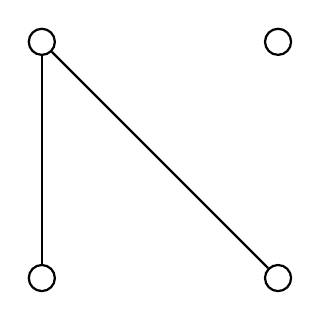
\begin{tikzpicture}[auto, node distance=3cm, every loop/.style={},
	thick,main node/.style={circle,draw,font=\sffamily\Large\bfseries}]
	
	\node[main node] (1) {};
	\node[main node] (2) [right of=1] {};
	\node[main node] (3) [below of=1] {};
	\node[main node] (4) [right of=3] {};
	
	\path[every node/.style={font=\sffamily\small}]
	(1)	edge node {} (3)
	(4) edge node {} (1);
	\end{tikzpicture}\quad\quad\quad
	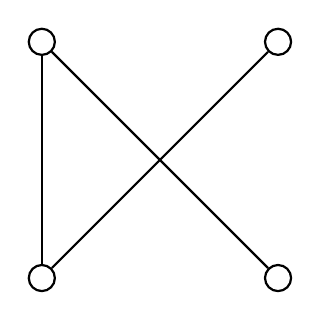
\begin{tikzpicture}[auto, node distance=3cm, every loop/.style={},
	thick,main node/.style={circle,draw,font=\sffamily\Large\bfseries}]
	
	\node[main node] (1) {};
	\node[main node] (2) [right of=1] {};
	\node[main node] (3) [below of=1] {};
	\node[main node] (4) [right of=3] {};
	
	\path[every node/.style={font=\sffamily\small}]
	(1)	edge node {} (3)
	(2) edge node {} (3)
	(4) edge node {} (1);
	\end{tikzpicture}\quad\quad\quad
	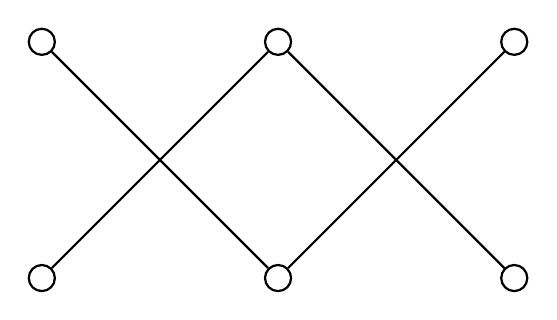
\begin{tikzpicture}[auto, node distance=3cm, every loop/.style={},
	thick,main node/.style={circle,draw,font=\sffamily\Large\bfseries}]
	
	\node[main node] (1) {};
	\node[main node] (2) [right of=1] {};
	\node[main node] (3) [right of=2] {};
	\node[main node] (4) [below of=1] {};
	\node[main node] (5) [right of=4] {};
	\node[main node] (6) [right of=5] {};
	
	\path[every node/.style={font=\sffamily\small}]
	(1)	edge node {} (5)
	(2) edge node {} (4)
	edge node {} (6)
	(3) edge node {} (5);
	\end{tikzpicture}
\end{center}
We find that only the graph in the middle is connected. For the graph on the right consider any vertex on the bottom, there is no path to the vertex above it. The graph on the left is has the upper right vertex isolated from the rest of the graph.

Any graph, connected or not, can be broken into connected components. To do this we simply take a vertex and every other vertex connected to it and call that one component, and then repeat with a vertex not in that component. This sort of breaking apart is nice as often we will prove things about connected graphs that are true about all graphs. For example if all components of a graph are planar then the entire graph must be planar, this will be proven below and it allows us to only deal with connected graphs.

\subsection{Contraction}
This is not a property, but rather an operation or action that we preform on a graph. Let us consider the following \gls{graph}.

\begin{center}
	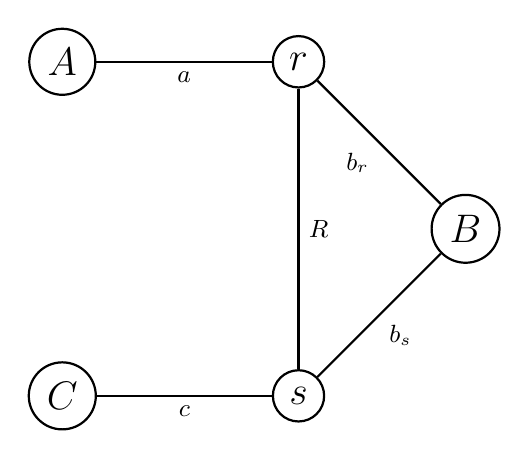
\begin{tikzpicture}[auto, node distance=3cm, every loop/.style={},
	thick,main node/.style={circle,draw,font=\sffamily\Large\bfseries}]
	
	\node[main node] (1) {$r$};
	\node[main node] (2) [below right of=1] {$B$};
	\node[main node] (3) [left of=1] {$A$};
	\node[main node] (4) [below left of=2] {$s$};
	\node[main node] (5) [left of=4] {$C$};
	
	\path[every node/.style={font=\sffamily\small}]
	(1) edge node {$R$} (4)
	edge node {$a$} (3)
	(2) edge node {$b_r$} (1)
	edge node {$b_s$} (4)
	(4) edge node {$c$} (5);
	\end{tikzpicture}
\end{center}

We wish to preform a \gls{contraction} on \gls{edge} $R$. To be clear all graph \glspl{contraction} are on \glspl{edge}. So we will make a new \gls{vertex}, $r\cdot s$ which has all the \glspl{edge} of $r$ and all the \glspl{edge} of $s$ except the \gls{edge} we are contracting across. In this case the \gls{edge} we are contracting across is $R$ and thus we get the following \gls{multigraph}.

\begin{center}
	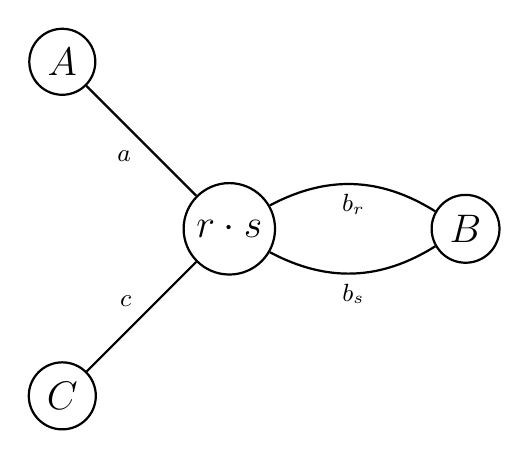
\begin{tikzpicture}[auto, node distance=3cm, every loop/.style={},
	thick,main node/.style={circle,draw,font=\sffamily\Large\bfseries}]
	
	\node[main node] (1) {$r\cdot s$};
	\node[main node] (2) [right of=1] {$B$};
	\node[main node] (3) [above left of=1] {$A$};
	\node[main node] (4) [below left of=1] {$C$};
	
	\path[every node/.style={font=\sffamily\small}]
	(1)	edge node {$a$} (3)
	(2) edge [bend right] node {$b_r$} (1)
	edge [bend left] node {$b_s$} (1)
	(4) edge node {$c$} (1);
	\end{tikzpicture}
\end{center}

This can then be reduced into a \gls{graph} again by simply treating $b_r$ and $b_s$ as the same edge. This operation is particularly important as we will prove that if a \gls{graph} is planar, then so is any \gls{graph} or \gls{multigraph} obtained by contracting an \gls{edge}.

\newpage

\section{Kuratowski's Theorem}
\begin{theorem}[Kuratowski's Theorem]
	A graph $G$ is planar if and only if it does not contain any subgraph $H$ such that a some series of edge contractions on $H$ would produce $K_5$ or $K_{3,3}$.
\end{theorem}

Here $K_5$ refers to the complete graph on 5 verticies, and $K_{3,3}$ is the complete bipartite graph with three verticies in both partitions. Drawings of both theses graphs are below with ($K_5$ on left and $K_{3,3}$ on right).
\begin{center}
	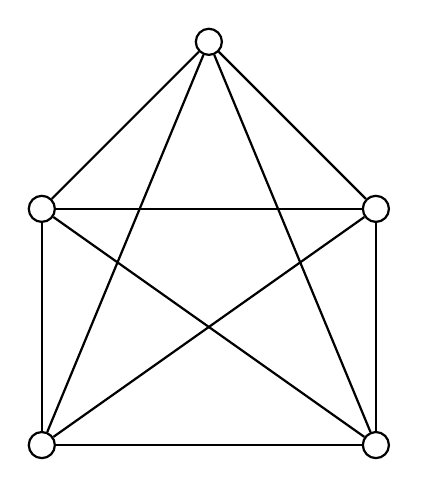
\begin{tikzpicture}[auto, node distance=3cm, every loop/.style={},
	thick,main node/.style={circle,draw,font=\sffamily\Large\bfseries}]
	
	\node[main node] (1) {};
	\node[main node] (2) [below left of=1] {};
	\node[main node] (3) [below right of=1] {};
	\node[main node] (4) [below of=2] {};
	\node[main node] (5) [below of=3] {};
	
	\path[every node/.style={font=\sffamily\small}]
	(1)	edge node {} (2)
	edge node {} (3)
	edge node {} (4)
	edge node {} (5)
	(2) edge node {} (3)
	edge node {} (4)
	edge node {} (5)
	(3) edge node {} (4)
	edge node {} (5)
	(4) edge node {} (5);
	\end{tikzpicture}
	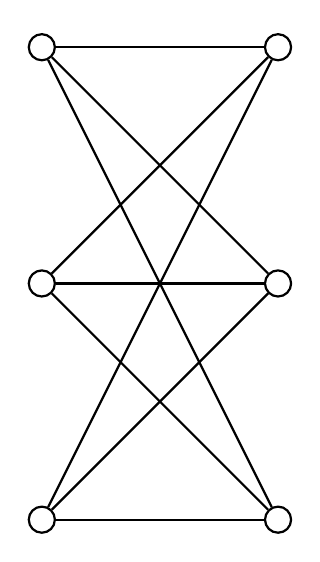
\begin{tikzpicture}[auto, node distance=3cm, every loop/.style={},
	thick,main node/.style={circle,draw,font=\sffamily\Large\bfseries}]
	
	\node[main node] (1) {};
	\node[main node] (2) [below of=1] {};
	\node[main node] (3) [below of=2] {};
	\node[main node] (4) [right of=1] {};
	\node[main node] (5) [below of=4] {};
	\node[main node] (6) [below of=5] {};
	
	\path[every node/.style={font=\sffamily\small}]
	(1)	edge node {} (4)
	edge node {} (5)
	edge node {} (6)
	(2)	edge node {} (4)
	edge node {} (5)
	edge node {} (6)
	(3)	edge node {} (4)
	edge node {} (5)
	edge node {} (6);
	\end{tikzpicture}
\end{center}

The basic sketch of the proof will be:
\begin{enumerate}
	\item Prove that $K_5$ and $K_3,3$ are not planar.
	\item Prove that if if a graph $G$ is planar than any graph obtained through an edge contraction is also planar.
	\item 
\end{enumerate}

\printnoidxglossary

\bibliographystyle{unsrt}
\bibliography{bibliography}

\end{document}